\documentclass[
BCOR0.7cm,							% Bindekorrektur, bspw. 1 cm
]
{scrbook}
\usepackage{ifpdf} 
\newif\ifpdf
\ifx\pdfoutput\undefined
	\pdffalse              	%normales LaTeX wird ausgef�hrt
\else
	\pdfoutput=1           
	\pdftrue               	%pdfLaTeX wird ausgef�hrt
\fi

\ifpdf
	%\usepackage{ae}        % Benutzen Sie nur
	%\usepackage{zefonts}  	% eines dieser Pakete
\else
	%%Normales LaTeX - keine speziellen Fontpackages notwendig
\fi

\ifpdf %%Einbindung von Grafiken mittels \includegraphics{datei}
	\usepackage[pdftex]{graphicx} %%Grafiken in pdfLaTeX
\else
	\usepackage[dvips]{graphicx} %%Grafiken und normales LaTeX
\fi


\ifpdf
	\pdfinfo
	{
    /Author (Karl Burkhart)                                
    /Title (Kodierrichtlinien)     
    /Subject (Kodierrichtlinien)                                    
    /Keywords (Kodierrichtlinien FH-Complete)
	}
\else			
\fi

\usepackage{listings} \lstset{numbers=left, numberstyle=\tiny, numbersep=5pt}
\lstset{language=tex} 


\usepackage[pdftex,colorlinks=true,urlcolor=blue,linkcolor=blue]{hyperref}
\usepackage[ngerman]{babel}		
\usepackage[T1]{fontenc}
\usepackage[latin9]{inputenc}
\usepackage{makeidx}
\usepackage{float}
\usepackage[small,bf]{caption}
\usepackage{fancyhdr}
\usepackage{amssymb,amsmath}
\usepackage{listings}
\usepackage{listings} \lstset{numbers=left, numberstyle=\tiny, numbersep=5pt} \lstset{language=Perl} 
\makeindex

\graphicspath{{../../images/}}

\setlength{\tolerance}{2000}
\setlength{\parindent}{0pt}
\setlength{\parskip}{1ex plus 0.5ex minus 0.2ex}
\addtolength{\textheight}{2cm}
\addtolength{\headheight}{2pt}
\setlength{\captionmargin}{20pt}
\setlength{\parindent}{0ex}
\floatstyle{plain}
\floatname{example}{Example}

\newfloat{example}{hbtp}{loe}[chapter]
\floatplacement{figure}{hbtp}
\floatplacement{table}{htbp}

\newcommand{\dollar}{\char36}

\newenvironment{info}[1]{
    \hspace{-10mm}
    \fbox{
        \begin{minipage}{1cm}
        
\includegraphics[width=1cm]{icon_info}
        \end{minipage}
        \begin{minipage}{14.5cm}
        #1
        \end{minipage}
    }
}

\newenvironment{achtung}[1]{
    \hspace{-10mm}
    \fbox{
        \begin{minipage}{1cm}
        
\includegraphics[width=1cm]{icon_achtung}
        \end{minipage}
        \begin{minipage}{14.5cm}
        #1
        \end{minipage}
    }
}

\newenvironment{halt}[1]{
    \hspace{-10mm}
    \fbox{
        \begin{minipage}{1cm}
        
\includegraphics[width=1cm]{icon_halt}
        \end{minipage}
        \begin{minipage}{14.5cm}
        #1
        \end{minipage}
    }
}

\newenvironment{idee}[1]{
    \hspace{-10mm}
    \fbox{
        \begin{minipage}{1cm}
        
\includegraphics[width=1cm]{icon_idee}
        \end{minipage}
        \begin{minipage}{14.5cm}
        #1
        \end{minipage}
    }
}


\setlength{\unitlength}{1mm}

\newenvironment{markier}[5]{
    
    \thicklines \put(#2,#3){\vector(#4,#5){5}} \thinlines
    \put(#2,#3){\circle*{5}}
    \put(#2,#3){\textcolor{black}{\circle{5}}\makebox(-10,0){\textcolor{white}{#1}}}


}


\hyphenation{gleich-zeitig para-meter}


\begin{document}

\ifpdf
	\DeclareGraphicsExtensions{.pdf,.jpg,.png}
\else
	\DeclareGraphicsExtensions{.eps}
\fi

\pagestyle{fancyplain}

% Titelseite einbinden
%
% Titelseite, Abstrakt, Danksagung und Inhaltsverzeichnis
%
%% eigene Titelseitengestaltung %%%%%%%%%%%%%%%%%%%%%%%%%%%%%%%%%%%%%%%    

\begin{titlepage}
\begin{center}
\vspace*{40mm} \huge Kodierrichtlinien\\
\vspace*{10mm}
\large \textsc{FH-Complete Technikum Wien}

\vfill 
\includegraphics[width=130mm]{fhcomplete}
	
\vfill \textsc{FH Technikum Wien}\\

Wien, \today
\end{center}
\end{titlepage}


\tableofcontents			% Inhaltsverzeichnis
%\frontmatter					% Vorspann (z.B. r�mische Seitenzahlen)
%\chapter{Einleitung}
\mainmatter						% Hauptteil

%% Kapitel Anfang %%%%%%%%%%%%%%%%%%%%%%%%%%%%%%%%%%%%%%%%%%%%%%%%%

\chapter{\"Ubersicht}
\section{Motivation}
Dieses Dokument wurde erstellt um eine einheitlich Enwicklungsumgebung zu schaffen und die Vorgaben der Entwickler zu erhalten.

Vorteile bei der Einhaltung der Richtlinien sind eine raschere Einarbeitung ins System sowie der Erweiterung von Programmteilen.

\newpage

\section{Entwicklungsumgebung}

Die Standard Entwicklungsumgebung am Technikum-Wien ist Eclipse PDT (PHP Development Tools Project) oder Netbeans.

\href{http://www.eclipse.org/pdt/}{http://www.eclipse.org/pdt/} (Stand 16.11.2012) \newline
\href{http://netbeans.org/features/php/}{http://netbeans.org/features/php/} (Stand 16.11.2012)

\newpage
\section{Ordnerhierarchie}

Ordnerhierarchie des FH-Complete Systems

\begin{figure}
	\centering
	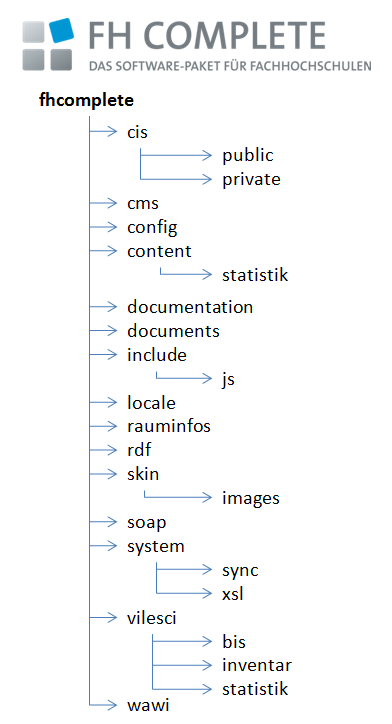
\includegraphics[width=0.65\textwidth]{Kodierrichtlinien_Ordnerhierarchie.png}
	\caption{Ordnerhierarchie von FH-Complete}
	\label{Ordnerhierarchie}
\end{figure}

\newpage
{\bf/cis:} Dateien speziell f\"ur das CIS System
\begin{itemize}
	\item{{\bf/public:} \"offentlich sichtbar}
	\item{{\bf/private:} Student/User muss eingeloggt sein um Content zu sehen (.htaccess)}
\end{itemize}

{\bf/cms:} Dateien f\"ur das CIS Content Management System und Document Management System

{\bf/config:} In diesem Ordner sind alle Konfigurationsdateien gespeichert (CIS, WAWI, VILESCI, Global) 

{\bf/content:} XUL Dateien FAS / TEMPUS / PLANNER
\begin{itemize}
	\item{{\bf/statistik:} Statistiken}
\end{itemize}

{\bf/dokumentation:} Dokumentation und Benutzerhandb\"ucher aller Systeme

{\bf/documents:}

{\bf/include:} Klassen und FH Spezifisches
\begin{itemize}
	\item{{\bf/js:} JavaScript Bibliotheken (JQuery)}
	\item{{\bf/tw:} Men\"ueintr\"age f\"ur Technikum Wien}
\end{itemize}
{\bf/locale:} Sprachdateien f\"ur FAS oder Sprachenmodul

{\bf/rauminfos:} Rauminfos aller R\"aume in HTML Files

{\bf/rdf:} RDF Files, zur PDF Erstellung ben\"otigt (Zeugnis, Bestellschein,..) 

{\bf/skin:} CSS Datein 
\begin{itemize}
	\item{{\bf/images:} Grafiken und Bilder f\"ur die Systeme}
\end{itemize}

{\bf/soap:} Alle Dateien f\"ur Webservices

{\bf/system:} Verwaltungsskripte 
\begin{itemize}
	\item{{\bf/sync:}}
	\item{{\bf/xsl:}}
\end{itemize}

{\bf/vilesci:} Dateien speziell f\"ur VILESCI
\begin{itemize}
	\item{{\bf/bis:} Bismeldungsrelevanten Daten}
	\item{{\bf/inventar:} Inventarprogramm}
	\item{{\bf/statistik:} Statistiken}
\end{itemize}

{\bf/wawi:} Files f\"ur WaWi

\section{Server\"ubersicht}

{\bf Sirene:} CIS, FHComplete, Moodle, Opus \newline
{\bf Fhctemp:} FAS, Tempus, Vilesci \newline
{\bf Theseus:} Datenbankserver (Postgres, MySQL) \newline
{\bf Calva:} Entwicklungsserver \newline
\chapter{Entwicklung-Software}
\section{Namensgebung}
Eine einheitliche Form der Namensgebung f\"ur Variablen, Konstanten und anderer Komponenten erleichter es dem Entwickler, den Code des anderen zu verstehen.

\subsection{Dateinamen}
Alle Dateinamen haben die f\"ur ihren Dateityp {\bf bestimmte Endung}. So haben z.B. HTML Dateien die Endung .html oder PHP Dateien .php. 
Es gibt jedoch Datentypen die eine {\bf eigene Schreibweise} haben. Hier eine Aufz\"ahlung der wichtigsten: \newline



\begin{tabular}{ll}
Klassen: & <klasse>.class.php \\
PHP-File: & <name>.php \\
HTML-File: & <name>.hmtl \\
RDF-File: & <name>.rdf \\
JavaScript: & <name>.js \\
CSS: & <name>.css \\
XUL: & <name>.xul \\
Config: & <name>.inc.php \\
\end{tabular}

Hierzu sind Endungen wie <name>.rdf.php oder <name>.js.php erlaubt. \newline
Es sind nur {\bf alphanumerische Zeichen, Underscores und Trennstriche} erlaubt. Beispiele f\"ur g\"ultige Namen sind: \newline
\begin{itemize}
\item studiengang.class.php
\item bestellung.rdf.php
\item tablesort.css
\item kontakt.js.php
\item ToDo\_CIS.html
\end{itemize}

\subsection{Variablen}
Alle Variablen m\"ussen mit {\bf Kleinbuchstaben beginnen} und der "`{\bf camelCaps}"' Namenskonventation folgen. Das bedeutet, wenn ein Variablenname aus mehereren
Namen besteht muss der Anfangsbuchstabe von jedem {\bf neuen Wort gro\ss{}geschrieben} werden. Repr\"{a}sentiert die Variable eine ID so wird die Endung ID mit \_ angef\"ugt. 
Variablennamen sind so {\bf kurz} und so {\bf verst\"andlich} wie m\"oglich
zu halten. Variablen wie "`\$i"' und "`\$j"' d\"urfen nur bei Loops verwendet werden.\\
{\bf Variablen in Klassen m\"ussen immer so hei\ss{}en wie sie in der Datenbank angelegt wurden.}
\begin{verbatim}
$anzahlVariablen
$datum
$person_id
\end{verbatim}

\subsection{Konstanten}
Pfade werden in Konstanten immer mit / beendet

\begin{verbatim}
define('SERVER_ROOT','http://calva.technikum-wien.at/');
\end{verbatim}

\subsection{Session Variablen}
Session Variablen die nur ein bestimmtes {\bf Modul} betreffen, werden folgenderma\ss en benannt: 
{\bf [Modulname] / [Name der Variable]}. Andere Session Variablen, die das ganze System betreffen werden ohne Modulnamen geschrieben. 
\begin{verbatim}
$_SESSION['cms/menu']
$_SESSION['wawi/user']
$_SESSION['user']
\end{verbatim}
Eine Session Variable wird {\bf immer klein geschrieben}. 

\subsection{Funktionen und Methoden}
Funktionsnamen m\"ussen immer mit einem {\bf Kleinbuchstaben beginnen}. Wenn eine Funktion aus mehreren Namen besteht, muss der Anfangsbuchstabe von jedem 
{\bf neuen Wort gro\ss geschrieben} werden. Funktionen und Methoden m\"ussen so {\bf klar} wie m\"oglich bezeichnet werden, damit anhand des Funktionsnamen jeder
versteht, wof\"ur diese bestimmt sind. Optionale \"Ubergabeparameter m\"ussen immer mit null initialisiert werden. \newline
Hier ein paar {\bf Beispiele} f\"ur g\"ultige Funktionsnamen:

\begin{verbatim}
getAllDetailsFromBestellung()
load()
saveTags($tag, $visible=null)
\end{verbatim}

\section{Kommentare}
Kommentare die nur eine Zeile lang sind sollen mit // beginnen. F\"ur Kommentare, die l\"anger als eine Zeile sind gilt als Start die /* Zeichenfolge und als Beendigung */. 

\subsection{Klassen}
Jede Klasse muss im Minimum einen {\bf Docblock} mit einer Beschreibung enthalten. \newline
Mit einem Docblock Kommentar bezeichnet man spezielle Kommentare, die sich automatisch generieren um PHP Abschnitte genauer zu kommentieren. Diese beginnen mit {\bf /**} und es k\"onnen spezielle tags wie @param oder @return benutzt werden. 

\begin{verbatim}
/**
 * Short description for class
 *
 * Long description for class (if any)...
 */
\end{verbatim}
 
\subsection{Funktionen und Methoden}
Jede Funktion oder Klassenmethode muss im Minimum einen {\bf Docblock} mit den folgenden Tags enthalten: {\bf Beschreibung, Parameter und R\"uckgabewerte}.
\begin{verbatim}
/**
 * Short description for the function
 *
 * Long description for the function (if any)...
 *
 * @param  array  $array  Description of array
 * @param  string $string Description of string
 * @return boolean 
 */
\end{verbatim}

\subsection{Variablen}
Jede Klassenvariable muss im Minimum einen {\bf Docblock} oder {\bf normalen} Kommentar enthalten welche den Typ der Variable ersichtlich macht. Wenn erforderlich kann dieser auch eine {\bf Beschreibung} der Variablen enthalten:
\begin{verbatim}
/**
 * Variable Description
 * @var array
 */
\end{verbatim}
\subsection{Programmkopf}

\begin{verbatim}
/* Copyright (C) 2011 Technikum-Wien
 *
 * This program is free software; you can redistribute it and/or modify
 * it under the terms of the GNU General Public License as
 * published by the Free Software Foundation; either version 2 of the
 * License, or (at your option) any later version.
 *
 * This program is distributed in the hope that it will be useful,
 * but WITHOUT ANY WARRANTY; without even the implied warranty of
 * MERCHANTABILITY or FITNESS FOR A PARTICULAR PURPOSE.  See the
 * GNU General Public License for more details.
 *
 * You should have received a copy of the GNU General Public License
 * along with this program; if not, write to the Free Software
 * Foundation, Inc., 59 Temple Place, Suite 330, Boston, MA 02111-1307,USA.
 *
 * Authors: Christian Paminger <christian.paminger@technikum-wien.at>,
 *     Andreas Oesterreicher <andreas.oesterreicher@technikum-wien.at> and
 *     Karl Burkhart <burkhart@technikum-wien.at>.
 */
\end{verbatim}
Zu beginn jedes Skriptes soll ganz oben der {\bf GNU Header} eingef\"ugt werden. \newline
Im {\bf Authors Block} werden nur Programmierer erw\"ahnt die das aktuelle File auch wirklich bearbeitet haben. 

\section{Programmierstil}
\subsection{Strings}
Ein String wird mit echo ausgegeben und sollte grunds\"atzlich mit {\bf einfachen Apostrophen}(single quotes) abgegrenzt werden. Dies hat den Vorteil, dass PHP Code im String {\bf nicht ausgef\"uhrt wird} und so z.B. HTML Ausgaben einfacher und schneller sind. Eine Folge von auszugebenden Strings kann mit Beistrich getrennt werden (anstatt mit . verkn\"upft), wodurch die Ausgabe beschleunigt wird

\begin{verbatim}
$message = 'Hello World';
echo '<div style="float: right;">',$message,'</div>';
echo '<div style="float: right;">'.$message.'</div>';
\end{verbatim}

\subsection{IF - ELSE}
Um Bl\"ocke zu gruppieren, k\"onnen {\bf zus\"atzliche Klammern} eingesetzt werden. Bei l\"angeren Bedingungen werden alle Bedingungen {\bf untereinander dargestellt}, um die Lesbarkeit zu erh\"ohen. Die \"offnende geschweifte Klammer wird immer in die {\bf n\"achste separate Zeile geschrieben}. Die abschlie\ss ende geschweifte Klammer erh\"alt ebenfalls immer eine separate Zeile. Jeder Code innerhalb der geschweiften Klammern muss {\bf einen Tabulator} (standardm\"a\ss ig vier Leerzeichen) einger\"uckt werden. \begin{verbatim}
if($user == 'Herbert')
{
   echo 'Hallo Herbert';
}
else
{
   echo 'Falscher User';
} 
\end{verbatim}
Bei sehr kurzen "`if-else"' Konstrukten kann auch der {\bf dreifach konditionale Operator} verwendet werden:
\begin{verbatim}
$sampleVar = isset($_GET['sampleVar']) ? $_GET['sampleVar'] : '';
\end{verbatim}
Gibt es nur eine ausf\"uhrende Zeile, so k\"onnen die geschweiften Klammern auch {\bf weggelassen werden}.
\begin{verbatim}
if($user == 'Herbert')
   echo 'Hallo Herbert';
else
   echo 'Falscher User';
\end{verbatim}

\subsection{Datenbankabfragen}
\begin{itemize}
\item Datenbankabfragen sind grunds\"atzlich \"uber die Datenbankklasse abzusetzen. 
\item Um SQL-Injections zu verhindern, sind die Paramter mittels der Funktion db\_add\_param zu escapen. 
(M\"ogliche \"Ubergabeparameter sind FHC\_INTEGER, FHC\_STRING und FHC\_BOOLEAN)
\item SQL Statements sind mit Strichpunkt abzuschlie\ss{}en.
\item Vor jedem Tabellennamen ist das entsprechende Schema anzugeben
\item Schl\"usselw\"orter (zB SELECT, WHERE, FROM, GROUP BY) sind gro\ss{} zu schreiben
\end{itemize}
\begin{verbatim}
$qry = "SELECT * FROM public.tbl_person WHERE 
person_id=".$db->db_add_param($person_id, FHC_INTEGER, false).';';
\end{verbatim}

Boolean Attribute sind ber die Datenbankklasse zu parsen um inkompatibilit\"aten mit verschiedenen DB-Systemen zu verhindern.

\begin{verbatim}
$aktiv = $db->db_parse_bool($row->aktiv);
\end{verbatim}

\subsection{HTML-Ausgaben}
HTML Attribute sollen generell mit doppelten Hochkomma umschlossen werden.
Variablen die innerhalb des HTML-Codes ausgegeben werden sind mit der Funktion convert\_html\_chars zu escapen. Dies ist vorallem wichtig bei Strings die den Typ Text oder varchar in der Datenbank haben. 

\begin{verbatim}
echo '<div style="float: right;">',$basis->convert_html_chars($message),'</div>';
\end{verbatim}


\subsection{Sonstiges}
\begin{itemize}
	\item {\bf Geschwungene Klammern} \\
	Um einen Block zu definieren werden die geschwungenen Klammern {\bf immer} in der neuen Zeile gesetzt. 
	\item {\bf Tabulator} \\
	Es wird immer wenn m\"oglich mit Tabulatoren einger\"uckt. Tabulatorbreite = 4 Leerzeichen. 
\end{itemize}
\chapter{Musterklasse}
\begin{verbatim}
<?php
/* Copyright (C) 2011 Technikum-Wien
 *
 * This program is free software; you can redistribute it and/or modify
 * it under the terms of the GNU General Public License as
 * published by the Free Software Foundation; either version 2 of the
 * License, or (at your option) any later version.
 *
 * This program is distributed in the hope that it will be useful,
 * but WITHOUT ANY WARRANTY; without even the implied warranty of
 * MERCHANTABILITY or FITNESS FOR A PARTICULAR PURPOSE.  See the
 * GNU General Public License for more details.
 *
 * You should have received a copy of the GNU General Public License
 * along with this program; if not, write to the Free Software
 * Foundation, Inc., 59 Temple Place, Suite 330, Boston, MA 02111-1307,USA.
 *
 * Authors: Christian Paminger <christian.paminger@technikum-wien.at>,
 *     Andreas Oesterreicher <andreas.oesterreicher@technikum-wien.at> and
 *     Karl Burkhart <burkhart@technikum-wien.at>.
 */
 require_once(dirname(__FILE__).'/basis_db.class.php');
\end{verbatim}
\begin{verbatim}
/**
 * Klasse Zweck liest und manipuliert Daten aus bis.tbl_zweck
 */ 
class zweck extends basis_db 
{
    /**
     * True wenn neues Objekt, False wenn Objekt schon vorhanden
     * @var boolean
     */
    public $new = true;

    /**
     * Zweck-Objekt Array
     * @var array
     */
    public $result = array();

    /**
     * Gibt alle Zweckbeschreibungen zurueck, bei Erfolg True
     *
     * @param  integer $id  Id die geladen warden soll, wenn keine id uebergeben wurde werden alle geladen
     * @return boolean
     */
    public function getAll($id = null)
    {
       return true; 
    }
}
?>
\end{verbatim}


\chapter{Code Reviews}
\underline{{\bf 20. Mai 2011 - abschlusspruefung.class.php}}
\begin{itemize}
	\item Getter und Setter
		\begin{itemize}
			\item {\bf Wichtige} Attribute protected
			\item Realisierbar mit {\bf \_\_set} und {\bf \_\_get}
		\end{itemize}
\end{itemize}
\begin{verbatim}
public function __set($name, $value)
{
   $this->vars[$name] = $value;
}
\end{verbatim}
\begin{itemize}
	\item Klasse soll alles erledigen
		\begin{itemize}
		\item Konstruktor setzt \$new = true
		\item Funktion load() setzt \$new = false
		\item Save() unterscheidet true oder false (insert oder update)
		\end{itemize}
\end{itemize}
\begin{itemize}
	\item Allgemein
		\begin{itemize}
		\item Immer require\_once() verwenden
		\item Im Skriptkopf nur den Autor vermerken, der File wirklich bearbeitet hat
		\item \"Uber Klasse Kommentarblock \newline
		\end{itemize}
\end{itemize}
\underline{{\bf 10. Juni 2011}}
\begin{itemize}
	\item Allgemein
		\begin{itemize}
		\item Ordnerstruktur verbessern		
			\begin{itemize}
			\item local/cms Dateien in -> local/[sprache] verschieben
			\end{itemize}
		\item Phrasenmodul	
			\begin{itemize}
			\item Gro\ss - Kleinschreibung bei Name z.B.: ['global/fehlerBeiDerParameteruebergabe']
			\item Keine Sonderzeichen in Name
			\end{itemize}
		\item Variablen	
			\begin{itemize}
			\item Kein \_ vor private oder protected Variablen
			\item Docblock Kommentare bei Variablen nicht ntig, Kommentar mit {\bf Datentyp in Datenbank} reicht
			\end{itemize}
		\end{itemize}
\end{itemize}
\newpage

\underline{{\bf 07. Oktober 2011 - rdf.class.php}}
\begin{itemize}
	\item SOAP
		\begin{itemize}
		\item username / passwort optional in WSDL
		\item Objekt Array -> Complextype wenn mehere Parameter \"ubergeben werden 
		\end{itemize}
	\item XUL
		\begin{itemize}
		\item menuitemID = Element-Modul z.B.: menuitem-projekt
		\item Die Trennung erfolgt mit -, da beim markieren davor und dannach abgebrochen wird
		\end{itemize}
	\item RDF
		\begin{itemize}
		\item kein {\bf /alle} mehr -> sondern http://www.technikum-wien.at/[Datenbankname]
		\end{itemize}
	\item Adressoperator \&
	\item statische Variablen
	\item Configs s\"aubern und global.conf [include] f\"ur globale Konfiguration bereitstellen \newline
\end{itemize}

\underline{{\bf 11. November 2011 - bestellung.php - Projekt zu Bestellung zuordnen}}
\begin{itemize}
	\item Anf\"uhrungszeichen bei echo
		\begin{itemize}
		\item Es sollen die Einfachen Anf\"uhrungszeichen verwendet werden ['] und zur Stringverkettung der Beistrich [,]
			\begin{verbatim}
			echo 'Username: ',$user,' eingeloggt'; 
			\end{verbatim}
		\end{itemize}
	\item Einfache Apostroph ['] in String escapen -> htmlentities => eigene Funktion bauen
	\item Magic Quotes -> deprecated
	\item Session Authentifizierung im CIS / Kalenderschnittstellen
	\item Cross Side Scripting Schw\"achen ausarbeiten \newline
\end{itemize}

\underline{{\bf 16. Dezember 2011 - addslashes - String escapen}}
\begin{itemize}
	\item Einfache Anf\"uhrungszeichen bei echo und doppelte f\"ur Eigenschaften 
	\item Eine funktion db\_null\_value soll in die DB Klasse implementiert werden 
	\begin{itemize}
		\item Bei einem leeren String wird null geschrieben
		\item es soll ein Parameter \$quote \"ubergeben werden(defaultwert true) -> wenn false wird nicht gequotet (f\"ur Integer) 
	\end{itemize}
	\item Daten die aus DB kommen, sollen mit escaped werden(doublequotes ["] werden escaped) -> Quellcode soll nicht ver\"anderbar werden - Hierf�r steht in der Basisklasse die funktion convert\_html\_chars zur Verf�gung
	\item ! Auch quoten bei Integerzahlen in DB query? !!\newline
\end{itemize}

\underline{{\bf 10. Februar 2012 Escapen von DB Parametern - functions.inc.php ausmisten }}
\begin{itemize}
	\item Zum Escapen von DB Parametern steht nun eine neue Funktion zur Verf�gung: \$db->db\_add\_param(\$var, \$type, \$nullable) 
	\item Boolean Parameter ueber DB-Klasse parsen, damit keine Probleme mit anderen Datenbanken auftreten. (zB t/f bei Postgres 0/1 bei MySQL)
	\begin{itemize}
		\item Boolean die aus der Datenbank gelesen werden, sollen durch die funktion \$db->db\_parse\_bool(\$var) geparst werden
		\item Boolean die in die Datenbank geschrieben werden, sollen die Funktion \$db->db\_add\_param(\$var, \$type, \$nullable) verwenden
	\end{itemize}
	\item functions.inc.php s\"aubern
	\begin{itemize}
		\item Datumsfunktionen in datum.class.php auslagern
		\item eventuelle Auslagerung der Authentifizierungsfunktionen in eine eigene Klasse\newline
	\end{itemize}
\end{itemize}
\underline{{\bf 09. August 2012 Strichpunkt bei SQL Statements }}
\begin{itemize}
		\item SQL Statements im Code sind mit Strichpunkt am Schluss abzuschlie\ss{}en
\end{itemize}

\underline{{\bf 08. November 2012 - XSS L\"ucken und WYSIWYG}}
\begin{itemize}
	\item XSS-L\"ucke im CIS wo es m\"oglich ist fremde Webseiten in den main Frame einzuschleusen
		\begin{itemize}
		\item L\"osung: \"Uberpr\"ufung ob APP\_ROOT in URL vorkommt - wenn nicht dann Seite nicht laden und Email an uns senden
		\end{itemize}
	\item In den LV Infos k\"onnen Tags wie <ul><li> eingegeben werden -> soll \"uberarbeitet werden
	\item Anstatt dass jedes Jahr das gesamte CIS ins Archiv kopiert wird, sollen nur mehr die LV Infos weggespeichert werden
	\item Im WYSWYG Editor können Tags eingegeben werden. Auch <script> Tags
		\begin{itemize}
		\item SaveHTML dar\"uberlaufen lassen
		\item vor Speichern in DB durch Methode Tags rausfiltern
		\end{itemize}
	\item EMail Signaturen sollen in Zukunft als Phrase ausgelagert werden -> Auch für Community leichter zum Editieren \newline
	\item N\"achstes Codereview: Basis Klasse und Stundenplanklasse (Zusammenhang zu anderen Klassen)
\end{itemize}

%\chapter{Review}
�ber den Button ''Review anfordern'' kann ein Review-Team benachrichtigt werden. 
Diese k�nnen den Content pr�fen und danach best�tigen. \\
Dazu wird ein eigener Button angezeigt, sofern die Berechtigung dazu vorhanden
ist. Beim Best�tigen des Contents (Review OK / Publish) wird dieser automatisch
auf sichtbar gesetzt.\\
\\ 
Pro Organisationseinheit k�nnen unterschiedliche Reviewer eingetragen werden. 
Wird f�r die aktuelle Organisationseinheit kein Reviewer gefunden, 
wird automatisch der dar�berliegende Reviewer verst�ndigt. 
Wenn im Tree �berhalb keiner gefunden wird, werden alle Reviewer benachrichtigt.\\
Der Reviewer kann im FAS �ber den Karteireiter Funktionen zugeteilt werden.
(Funktion: review)

%\chapter{Dokumentenmanagement}
Das CMS System ist mit einem Dokumentenmanagementsystem gekoppelt. 
Klickt man auf das Symbol zum Einf�gen eines Links oder eines Bildes 
erh�lt man neben dem Eingabefeld f�r die URL ein kleines Symbol (1).
\begin{figure}
	\begin{center}
    \begin{picture}(56,45)
			\put(0,0){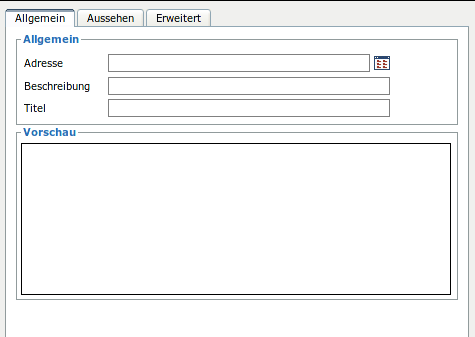
\includegraphics[height=40mm, width=56mm]{dms_erweitert_icon.png}}
			\markier{1}{52}{39}{-1}{-1}
		\end{picture}
    \caption{Dokumentenauswahl}
		\label{Dokumentenauswahl}
  \end{center}
\end{figure}

Hier gelangt man in das Dokumentenmanagementsystem.
Dokumente k�nnen hier hochgeladen und Kategorien zugeordnet werden. 
Mit einem klick auf den Namen wird die Datei ausgew�hlt und in den Editor eingef�gt.
\section{Hochladen von Dateien}
- Kategorie ausw�hlen\\
- "Datei hochladen" klicken\\
- im unteren Teil wird ein Formular angezeigt. Hier kann die Datei gesucht und
hochgeladen werden. \\
\section{Neue Version hochladen}
- Datei suchen\\
- Erweitert->Neue Version hochladen\\
- Datei ausw�hlen und hochladen\\

\section{Kategorien}
Damit die Dokumente nicht bunt durcheinandergemisch sind, k�nnen diese in
Kategorien zusammengefasst werden. Ein Dokument kann immer nur einer Kategorie
zugewiesen sein.

\section{Zugriffsrechte}
Der Zugriff auf Dokumente wird �ber die Kategorien gesteuert.\\
Zu jeder Kategorie k�nnen Gruppen zugeordnet werden. Die Mitglieder dieser Gruppe haben
dann Zugriff auf die Dokumente innerhalb dieser Kategorie. Die Rechte werden an die
darunterliegenden Kategorien vererbt.\\
Wenn keine Gruppenzuordnung f�r die Kategorie oder �bergeordneten Kategorien vorhanden ist, dann ist die Datei frei f�r alle zug�nglich.\\
\\
Eine Ausnahme stellen die Projektdokumente dar. Sobald ein Dokument zu einem Projekt zugeordnet ist, ist dieses Dokument nur noch von den Personen einsehbar, welche dem entsprechenden Projekt zugeordnet sind.\\
\\
F�r Administratoren kann die Berechtigung 'basis/dms' vergeben werden. Mit diesem Recht kann auf alle Dokumente zugegriffen werden.\\
\\
Gesperrte Kategorien werden im DMS System mit einem Schloss Symbol versehen.
%\chapter{Administratives}
\section{DMS}
Die Dateien werden im DMS\_PATH abgelegt. Die Berechtigung wird f�r die Gruppe
"dms" gesetzt! Diese Gruppe muss am Server vorhanden sein, da es sonst 
m�glicherweise zu problemen beim Zugriff kommt.\\
\section{Import}
Ist die Datei gr��er als 15 MB (PHP upload\_max\_filesize) kann sie �ber den
Import Ordner hochgeladen werden. Die Datei wird vorher per WinSCP etc in den
Import Ordner (siehe Config) kopiert. Die Dateien des Import Ordners werden unterhalb des Formulars angezeigt und 
k�nnen mittels ''Hochladen'' ins DMS �bernommen werden
\section{Men� Addons}
Include Addons befinden sich unter /cms/menu/. Pro Addon gibt es ein eigenes
File. Darin befindet sich eine Klasse die von der Klasse menu\_addon abgeleitet
ist. Diese Klasse bef�llt Variablen der Basisklasse welche dann ausgegeben werden.
\section{Startpunkt des CMS}
Der Content bei dem das Men� im CIS beginnt kann �ber eine Config Variable
definiert werden.


%% Kapitel Ende   %%%%%%%%%%%%%%%%%%%%%%%%%%%%%%%%%%%%%%%%%%%%%%%%%
%\appendix							% Beginn des Anhangs
%\chapter{Schluss}
%\listoftables					% Tabellenverzeichnis
%\listoffigures				% Abbildungsverzeichnis

\end{document}


